%% LyX 2.2.3 created this file.  For more info, see http://www.lyx.org/.
%% Do not edit unless you really know what you are doing.
\documentclass[ruled]{article}
\usepackage{courier}
\usepackage[T1]{fontenc}
\usepackage[latin9]{inputenc}
\usepackage[letterpaper]{geometry}
\geometry{verbose}
\usepackage{color}
\usepackage{url}
\usepackage{algorithm2e}
\usepackage{amsmath}
\usepackage{amssymb}
\usepackage{titlesec}
\newcommand{\sectionbreak}{\clearpage}
\usepackage{graphicx}
\usepackage[export]{adjustbox}
\graphicspath{ {./images/} }
\usepackage{listings}
\usepackage{pdfpages}
\usepackage[unicode=true,
 bookmarks=false,
 breaklinks=false,pdfborder={0 0 1},backref=section,colorlinks=true]
 {hyperref}

\makeatletter

%%%%%%%%%%%%%%%%%%%%%%%%%%%%%% LyX specific LaTeX commands.
\providecommand{\LyX}{\texorpdfstring%
  {L\kern-.1667em\lower.25em\hbox{Y}\kern-.125emX\@}
  {LyX}}
%% Special footnote code from the package 'stblftnt.sty'
%% Author: Robin Fairbairns -- Last revised Dec 13 1996
\let\SF@@footnote\footnote
\def\footnote{\ifx\protect\@typeset@protect
    \expandafter\SF@@footnote
  \else
    \expandafter\SF@gobble@opt
  \fi
}
\expandafter\def\csname SF@gobble@opt \endcsname{\@ifnextchar[%]
  \SF@gobble@twobracket
  \@gobble
}
\edef\SF@gobble@opt{\noexpand\protect
  \expandafter\noexpand\csname SF@gobble@opt \endcsname}
\def\SF@gobble@twobracket[#1]#2{}

\@ifundefined{date}{}{\date{}}
%%%%%%%%%%%%%%%%%%%%%%%%%%%%%% User specified LaTeX commands.
\definecolor{mygreen}{rgb}{0,0.6,0}
\definecolor{mygray}{rgb}{0.5,0.5,0.5}
\definecolor{mymauve}{rgb}{0.58,0,0.82}

\makeatother

\usepackage{listings}
\lstset{backgroundcolor={\color{white}},
basicstyle={\footnotesize\ttfamily},
breakatwhitespace=false,
breaklines=true,
captionpos=b,
commentstyle={\color{mygreen}},
deletekeywords={...},
escapeinside={\%*}{*)},
extendedchars=true,
frame=shadowbox,
keepspaces=true,
keywordstyle={\color{blue}},
language=Python,
morekeywords={*,...},
numbers=none,
numbersep=5pt,
numberstyle={\tiny\color{mygray}},
rulecolor={\color{black}},
showspaces=false,
showstringspaces=false,
showtabs=false,
stepnumber=1,
stringstyle={\color{mymauve}},
tabsize=2}

 
\begin{document}

\global\long\def\reals{\mathbf{R}}
 \global\long\def\integers{\mathbf{Z}}
\global\long\def\naturals{\mathbf{N}}
 \global\long\def\rationals{\mathbf{Q}}
\global\long\def\ca{\mathcal{A}}
\global\long\def\cb{\mathcal{B}}
 \global\long\def\cc{\mathcal{C}}
 \global\long\def\cd{\mathcal{D}}
\global\long\def\ce{\mathcal{E}}
\global\long\def\cf{\mathcal{F}}
\global\long\def\cg{\mathcal{G}}
\global\long\def\ch{\mathcal{H}}
\global\long\def\ci{\mathcal{I}}
\global\long\def\cj{\mathcal{J}}
\global\long\def\ck{\mathcal{K}}
\global\long\def\cl{\mathcal{L}}
\global\long\def\cm{\mathcal{M}}
\global\long\def\cn{\mathcal{N}}
\global\long\def\co{\mathcal{O}}
\global\long\def\cp{\mathcal{P}}
\global\long\def\cq{\mathcal{Q}}
\global\long\def\calr{\mathcal{R}}
\global\long\def\cs{\mathcal{S}}
\global\long\def\ct{\mathcal{T}}
\global\long\def\cu{\mathcal{U}}
\global\long\def\cv{\mathcal{V}}
\global\long\def\cw{\mathcal{W}}
\global\long\def\cx{\mathcal{X}}
\global\long\def\cy{\mathcal{Y}}
\global\long\def\cz{\mathcal{Z}}
\global\long\def\ind#1{1(#1)}
\global\long\def\pr{\mathbb{P}}

\global\long\def\ex{\mathbb{E}}
\global\long\def\var{\textrm{Var}}
\global\long\def\cov{\textrm{Cov}}
\global\long\def\sgn{\textrm{sgn}}
\global\long\def\sign{\textrm{sign}}
\global\long\def\kl{\textrm{KL}}
\global\long\def\law{\mathcal{L}}
\global\long\def\eps{\varepsilon}
\global\long\def\convd{\stackrel{d}{\to}}
\global\long\def\eqd{\stackrel{d}{=}}
\global\long\def\del{\nabla}
\global\long\def\loss{\ell}
\global\long\def\tr{\operatorname{tr}}
\global\long\def\trace{\operatorname{trace}}
\global\long\def\diag{\text{diag}}
\global\long\def\rank{\text{rank}}
\global\long\def\linspan{\text{span}}
\global\long\def\proj{\text{Proj}}
\global\long\def\argmax{\operatornamewithlimits{arg\, max}}
\global\long\def\argmin{\operatornamewithlimits{arg\, min}}
\global\long\def\bfx{\mathbf{x}}
\global\long\def\bfy{\mathbf{y}}
\global\long\def\bfl{\mathbf{\lambda}}
\global\long\def\bfm{\mathbf{\mu}}
\global\long\def\calL{\mathcal{L}}
\global\long\def\vw{\boldsymbol{w}}
\global\long\def\vx{\boldsymbol{x}}
\global\long\def\vxi{\boldsymbol{\xi}}
\global\long\def\valpha{\boldsymbol{\alpha}}
\global\long\def\vbeta{\boldsymbol{\beta}}
\global\long\def\vsigma{\boldsymbol{\sigma}}
\global\long\def\vmu{\boldsymbol{\mu}}
\global\long\def\vtheta{\boldsymbol{\theta}}
\global\long\def\vd{\boldsymbol{d}}
\global\long\def\vs{\boldsymbol{s}}
\global\long\def\vt{\boldsymbol{t}}
\global\long\def\vh{\boldsymbol{h}}
\global\long\def\ve{\boldsymbol{e}}
\global\long\def\vf{\boldsymbol{f}}
\global\long\def\vg{\boldsymbol{g}}
\global\long\def\vz{\boldsymbol{z}}
\global\long\def\vk{\boldsymbol{k}}
\global\long\def\va{\boldsymbol{a}}
\global\long\def\vb{\boldsymbol{b}}
\global\long\def\vv{\boldsymbol{v}}
\global\long\def\vy{\boldsymbol{y}}



\title{Machine Learning and Computational Statistics\\
Hypothesis Space $\&$ Statistical Learning Theory}

\maketitle
\textbf{Note}: This document consists of concepts and exercises related to hypothesis space and statistical learning theories.

\section{Learning} % This is new.
\subsection{Learning Objectives}
\begin{enumerate}
\item Identify the input, action, and outcome spaces for a given machine learning problem.
\item Provide an example for which the action space and outcome spaces are the same and one for which they are different.
\item Explain the relationships between the decision function, the loss function, the input space, the action space, and the outcome space.
\item Define the risk of a decision function and a Bayes decision function.
\item Provide example decision problems for which the Bayes risk is 0 and the Bayes risk is nonzero.
\item Know the Bayes decision functions for square loss and multiclass 0/1 loss.
\item Define the empirical risk for a decision function and the empirical risk minimizer.
\item Explain what a hypothesis space is, and how it can be used with constrained empirical risk minimization to control overfitting.
\end{enumerate}

\subsection{Concepts}
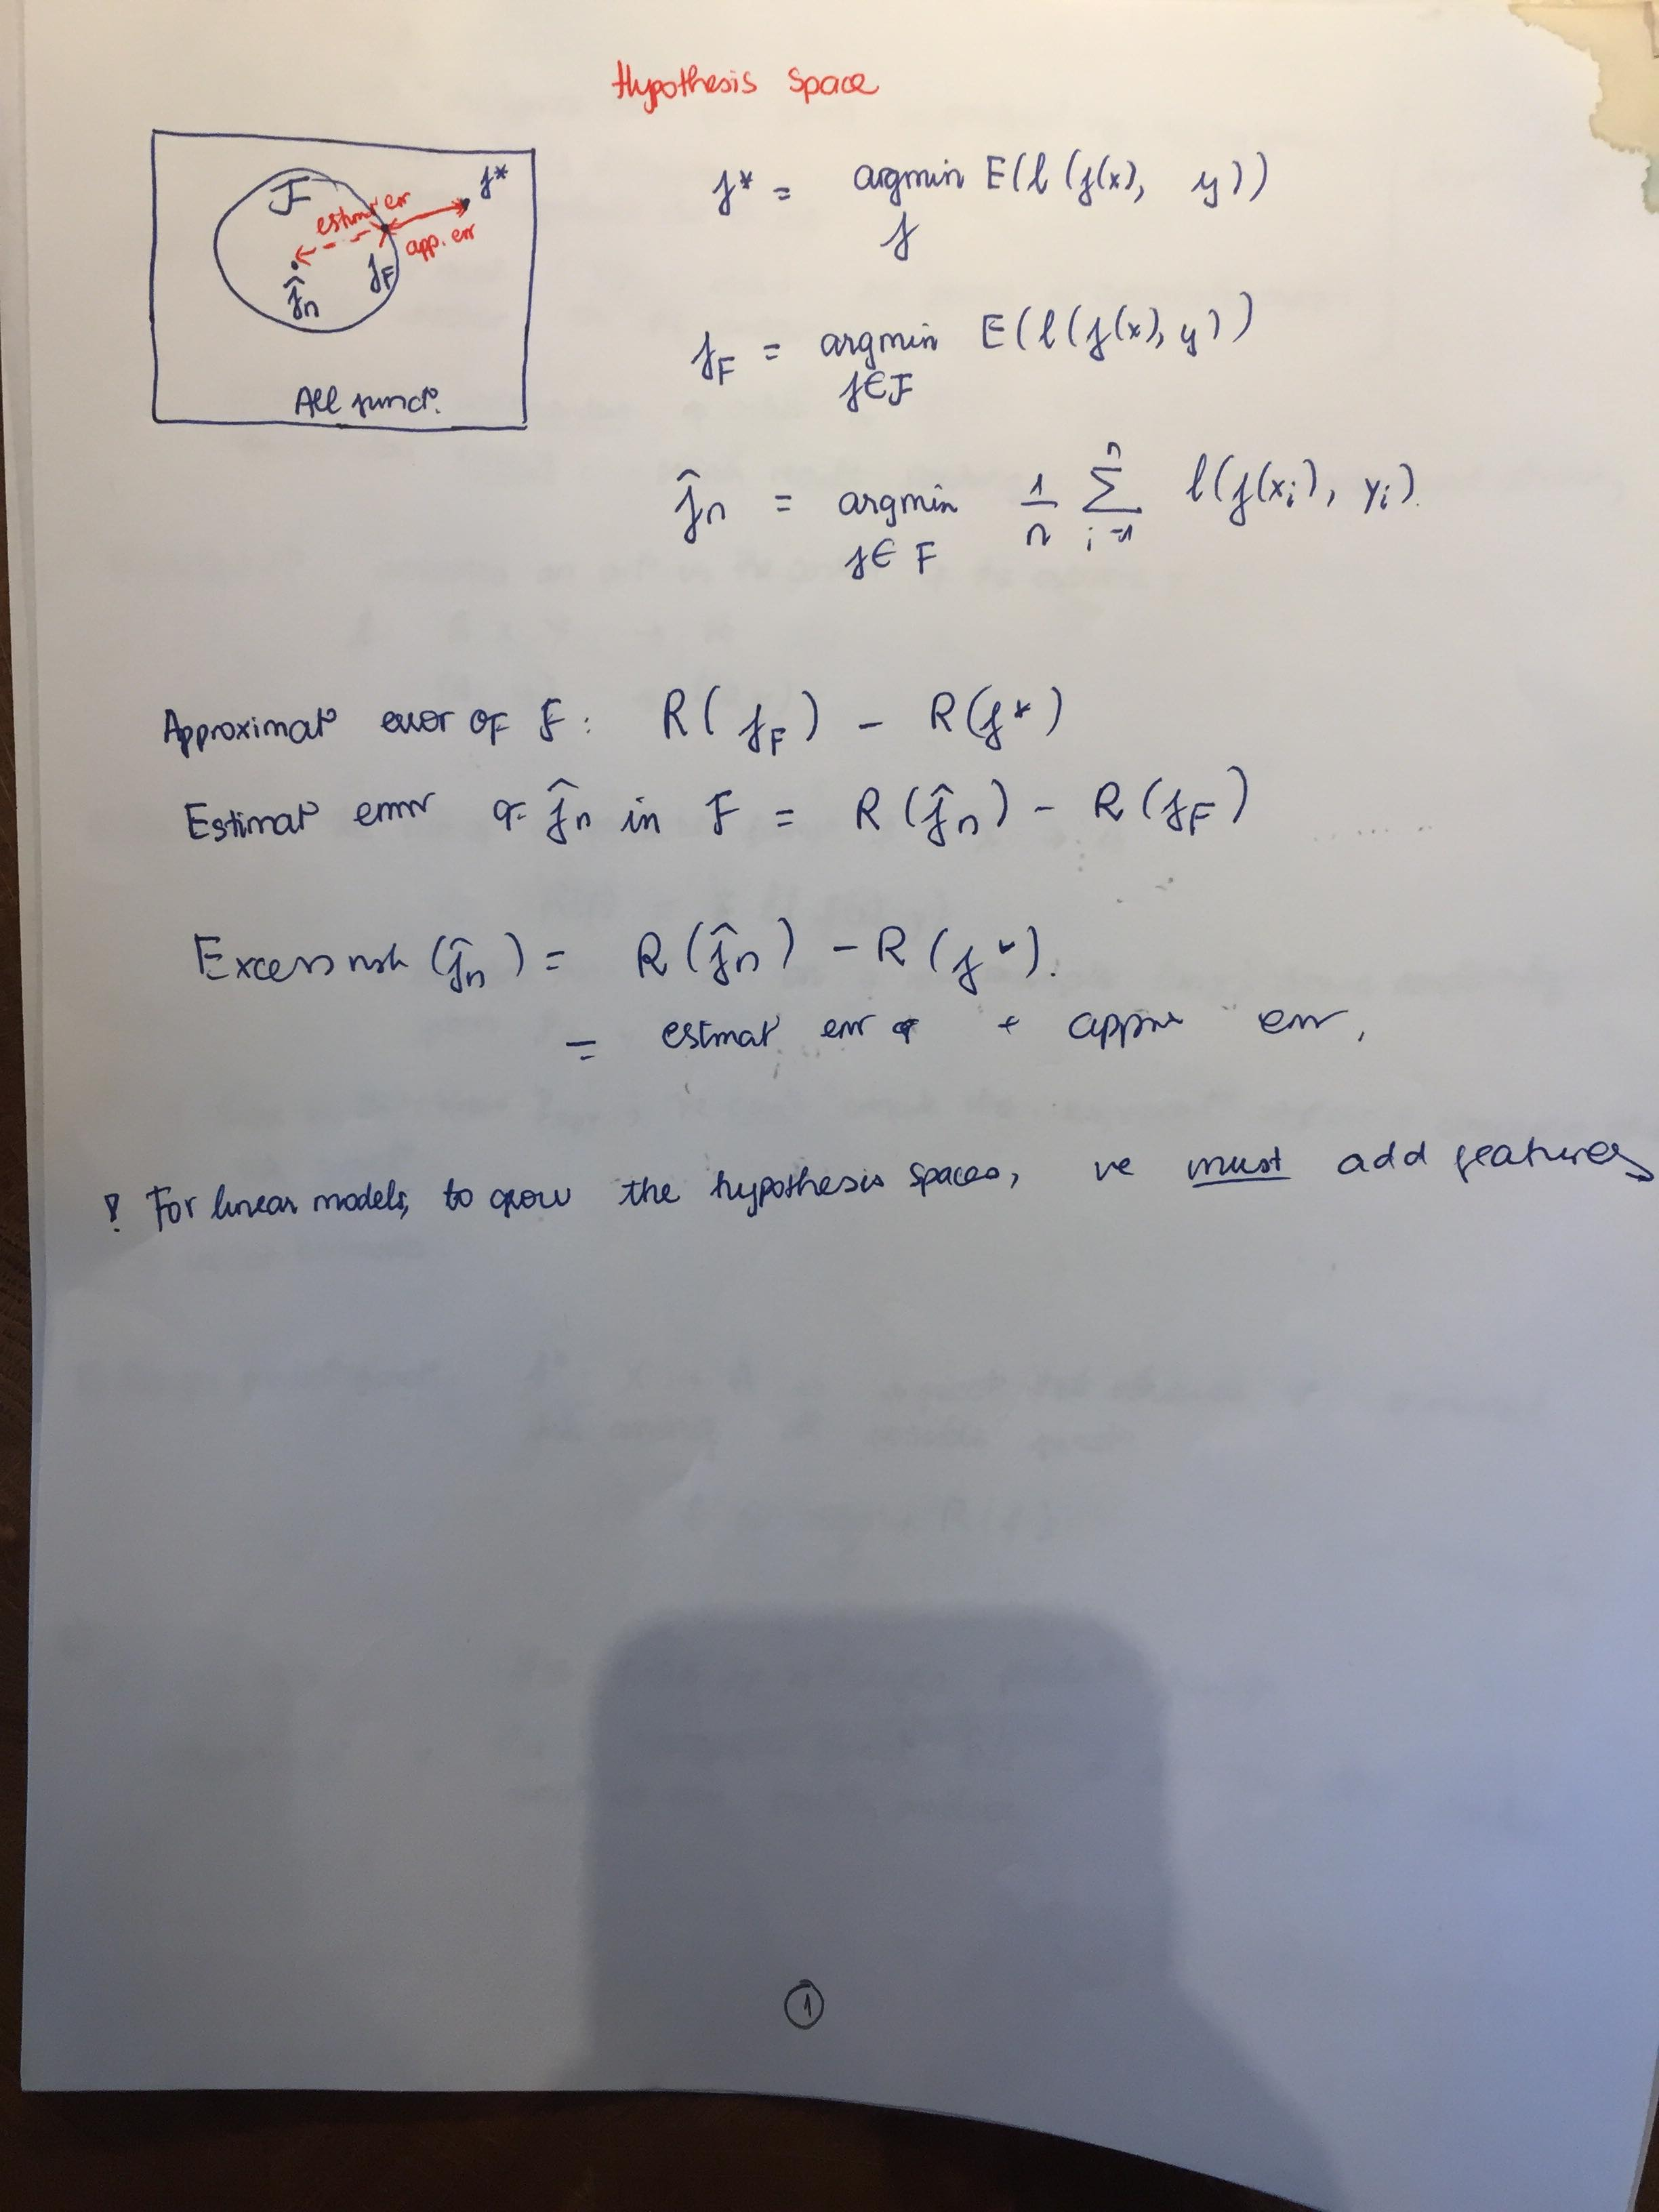
\includegraphics[max size={\textwidth}{\textheight}]{HypoSpace1.jpg} \\

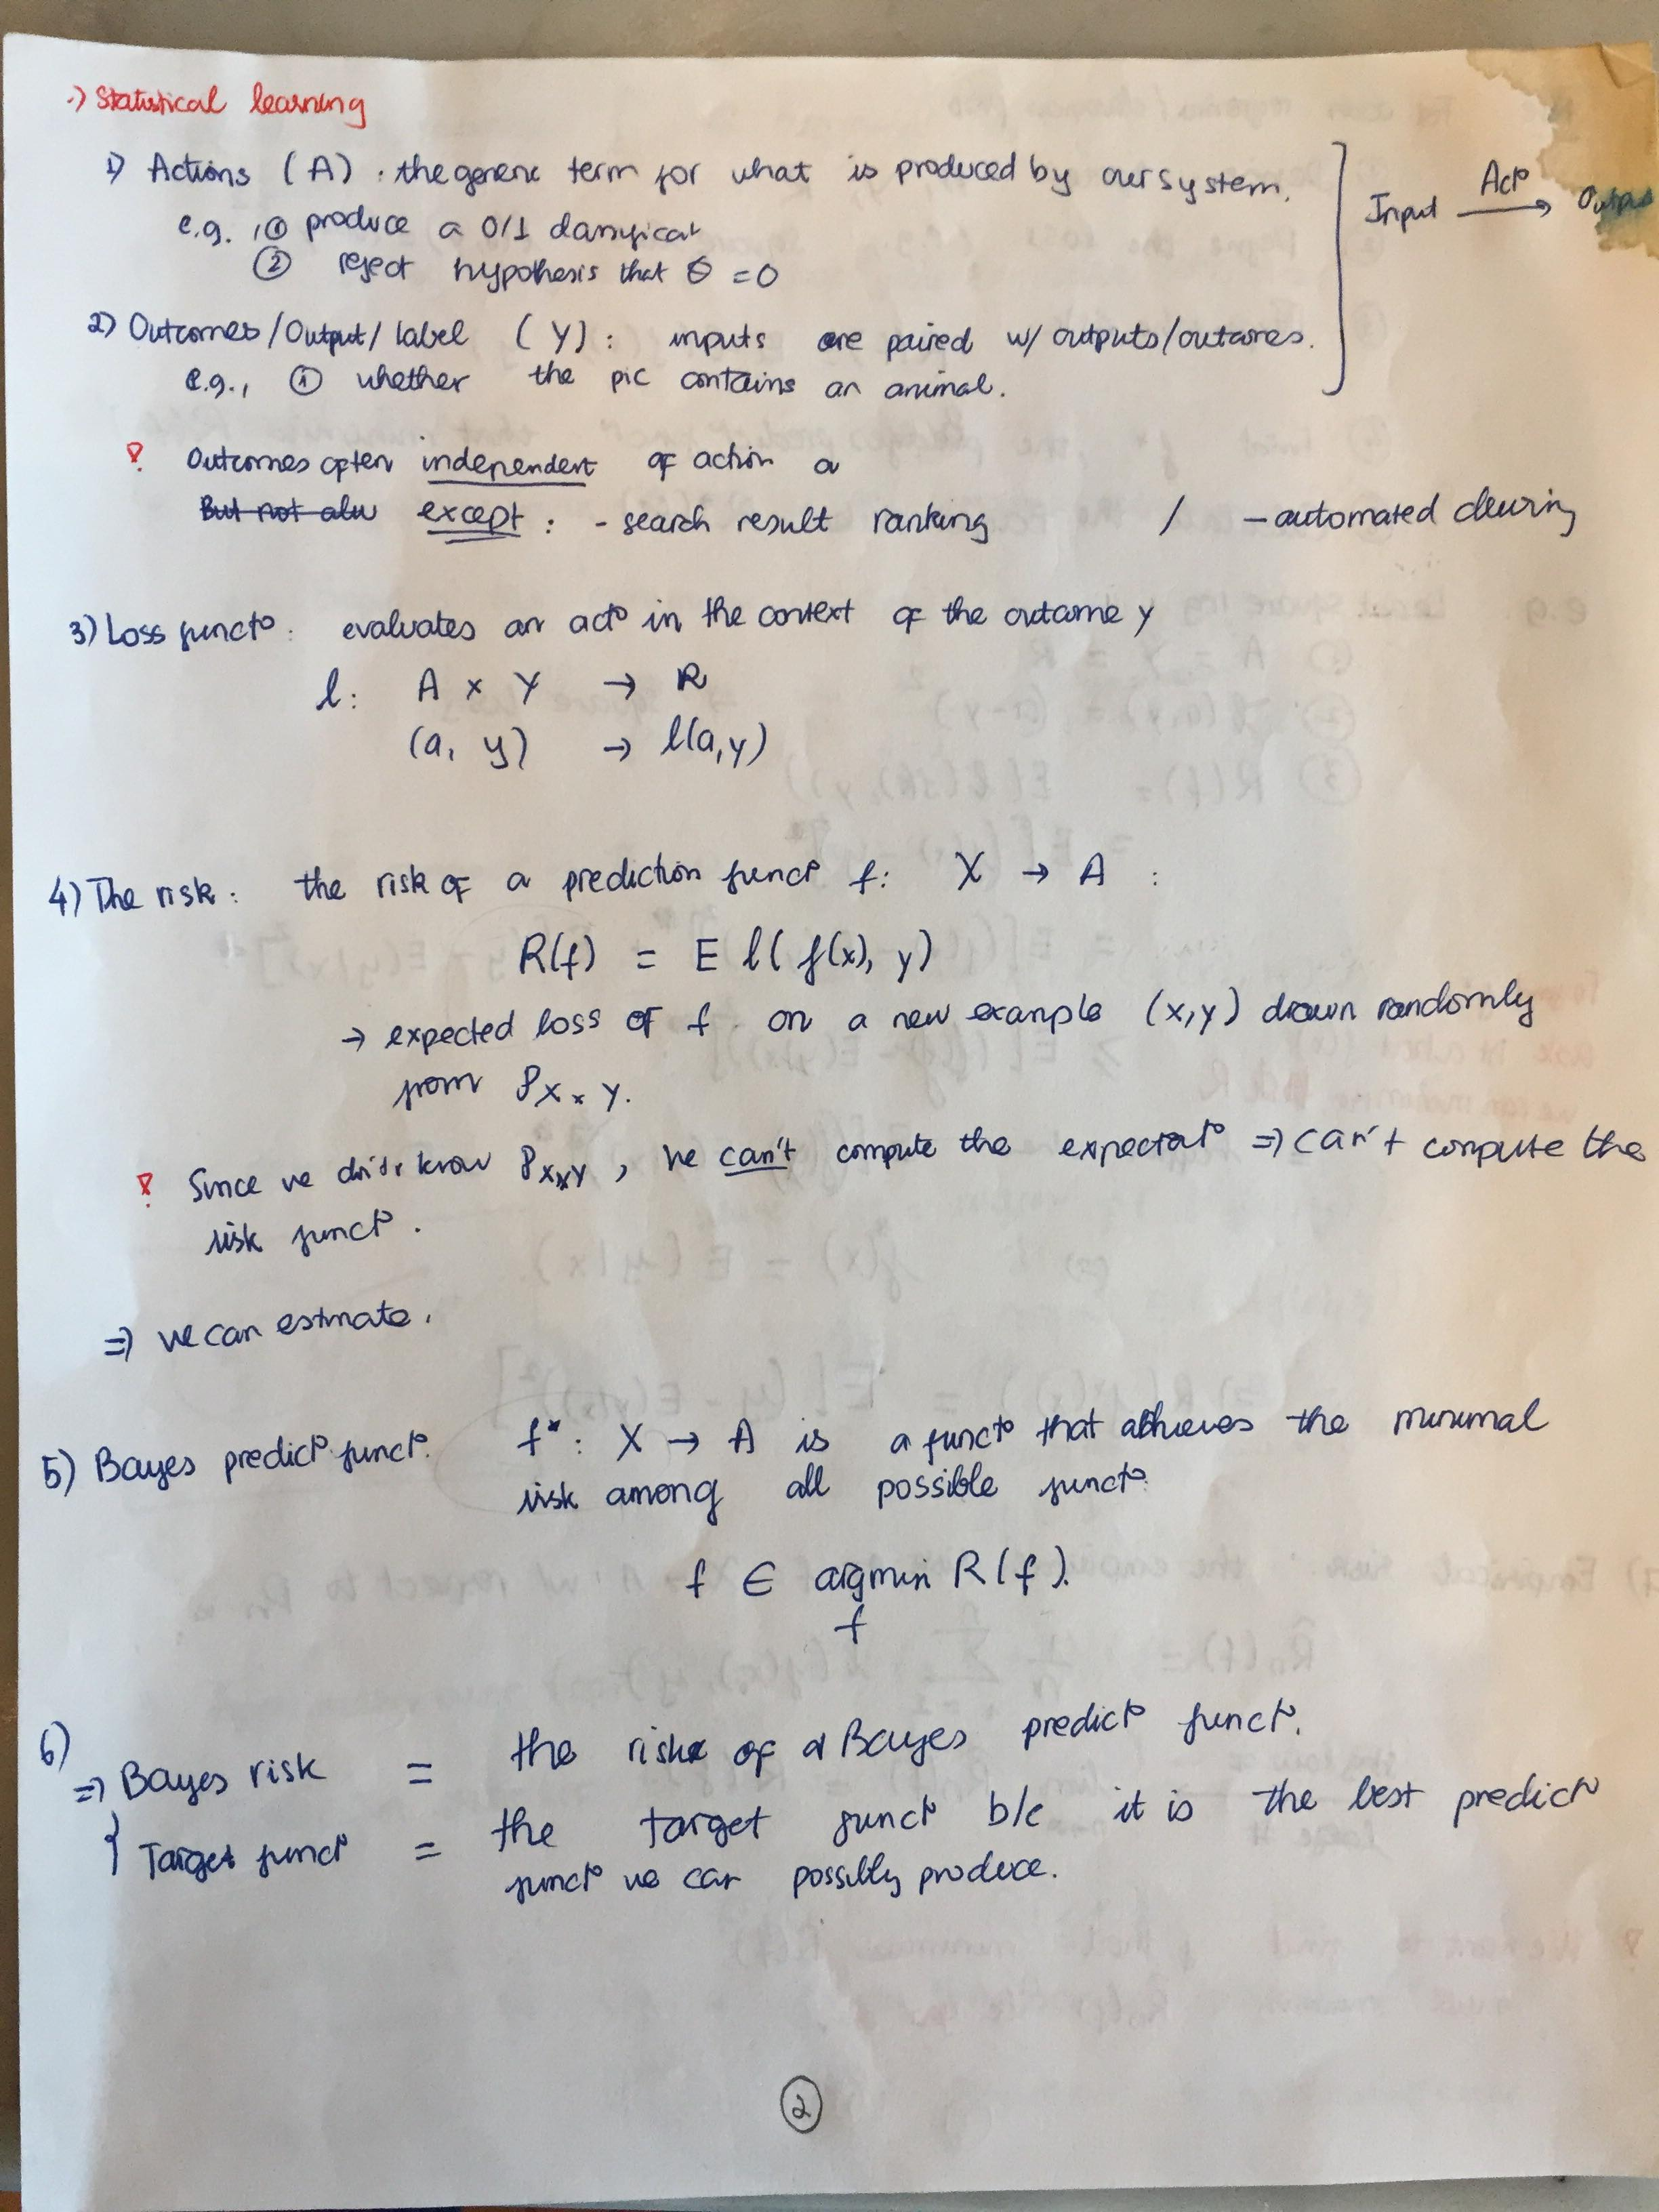
\includegraphics[max size={\textwidth}{\textheight}]{HypoSpace2.jpg} \\
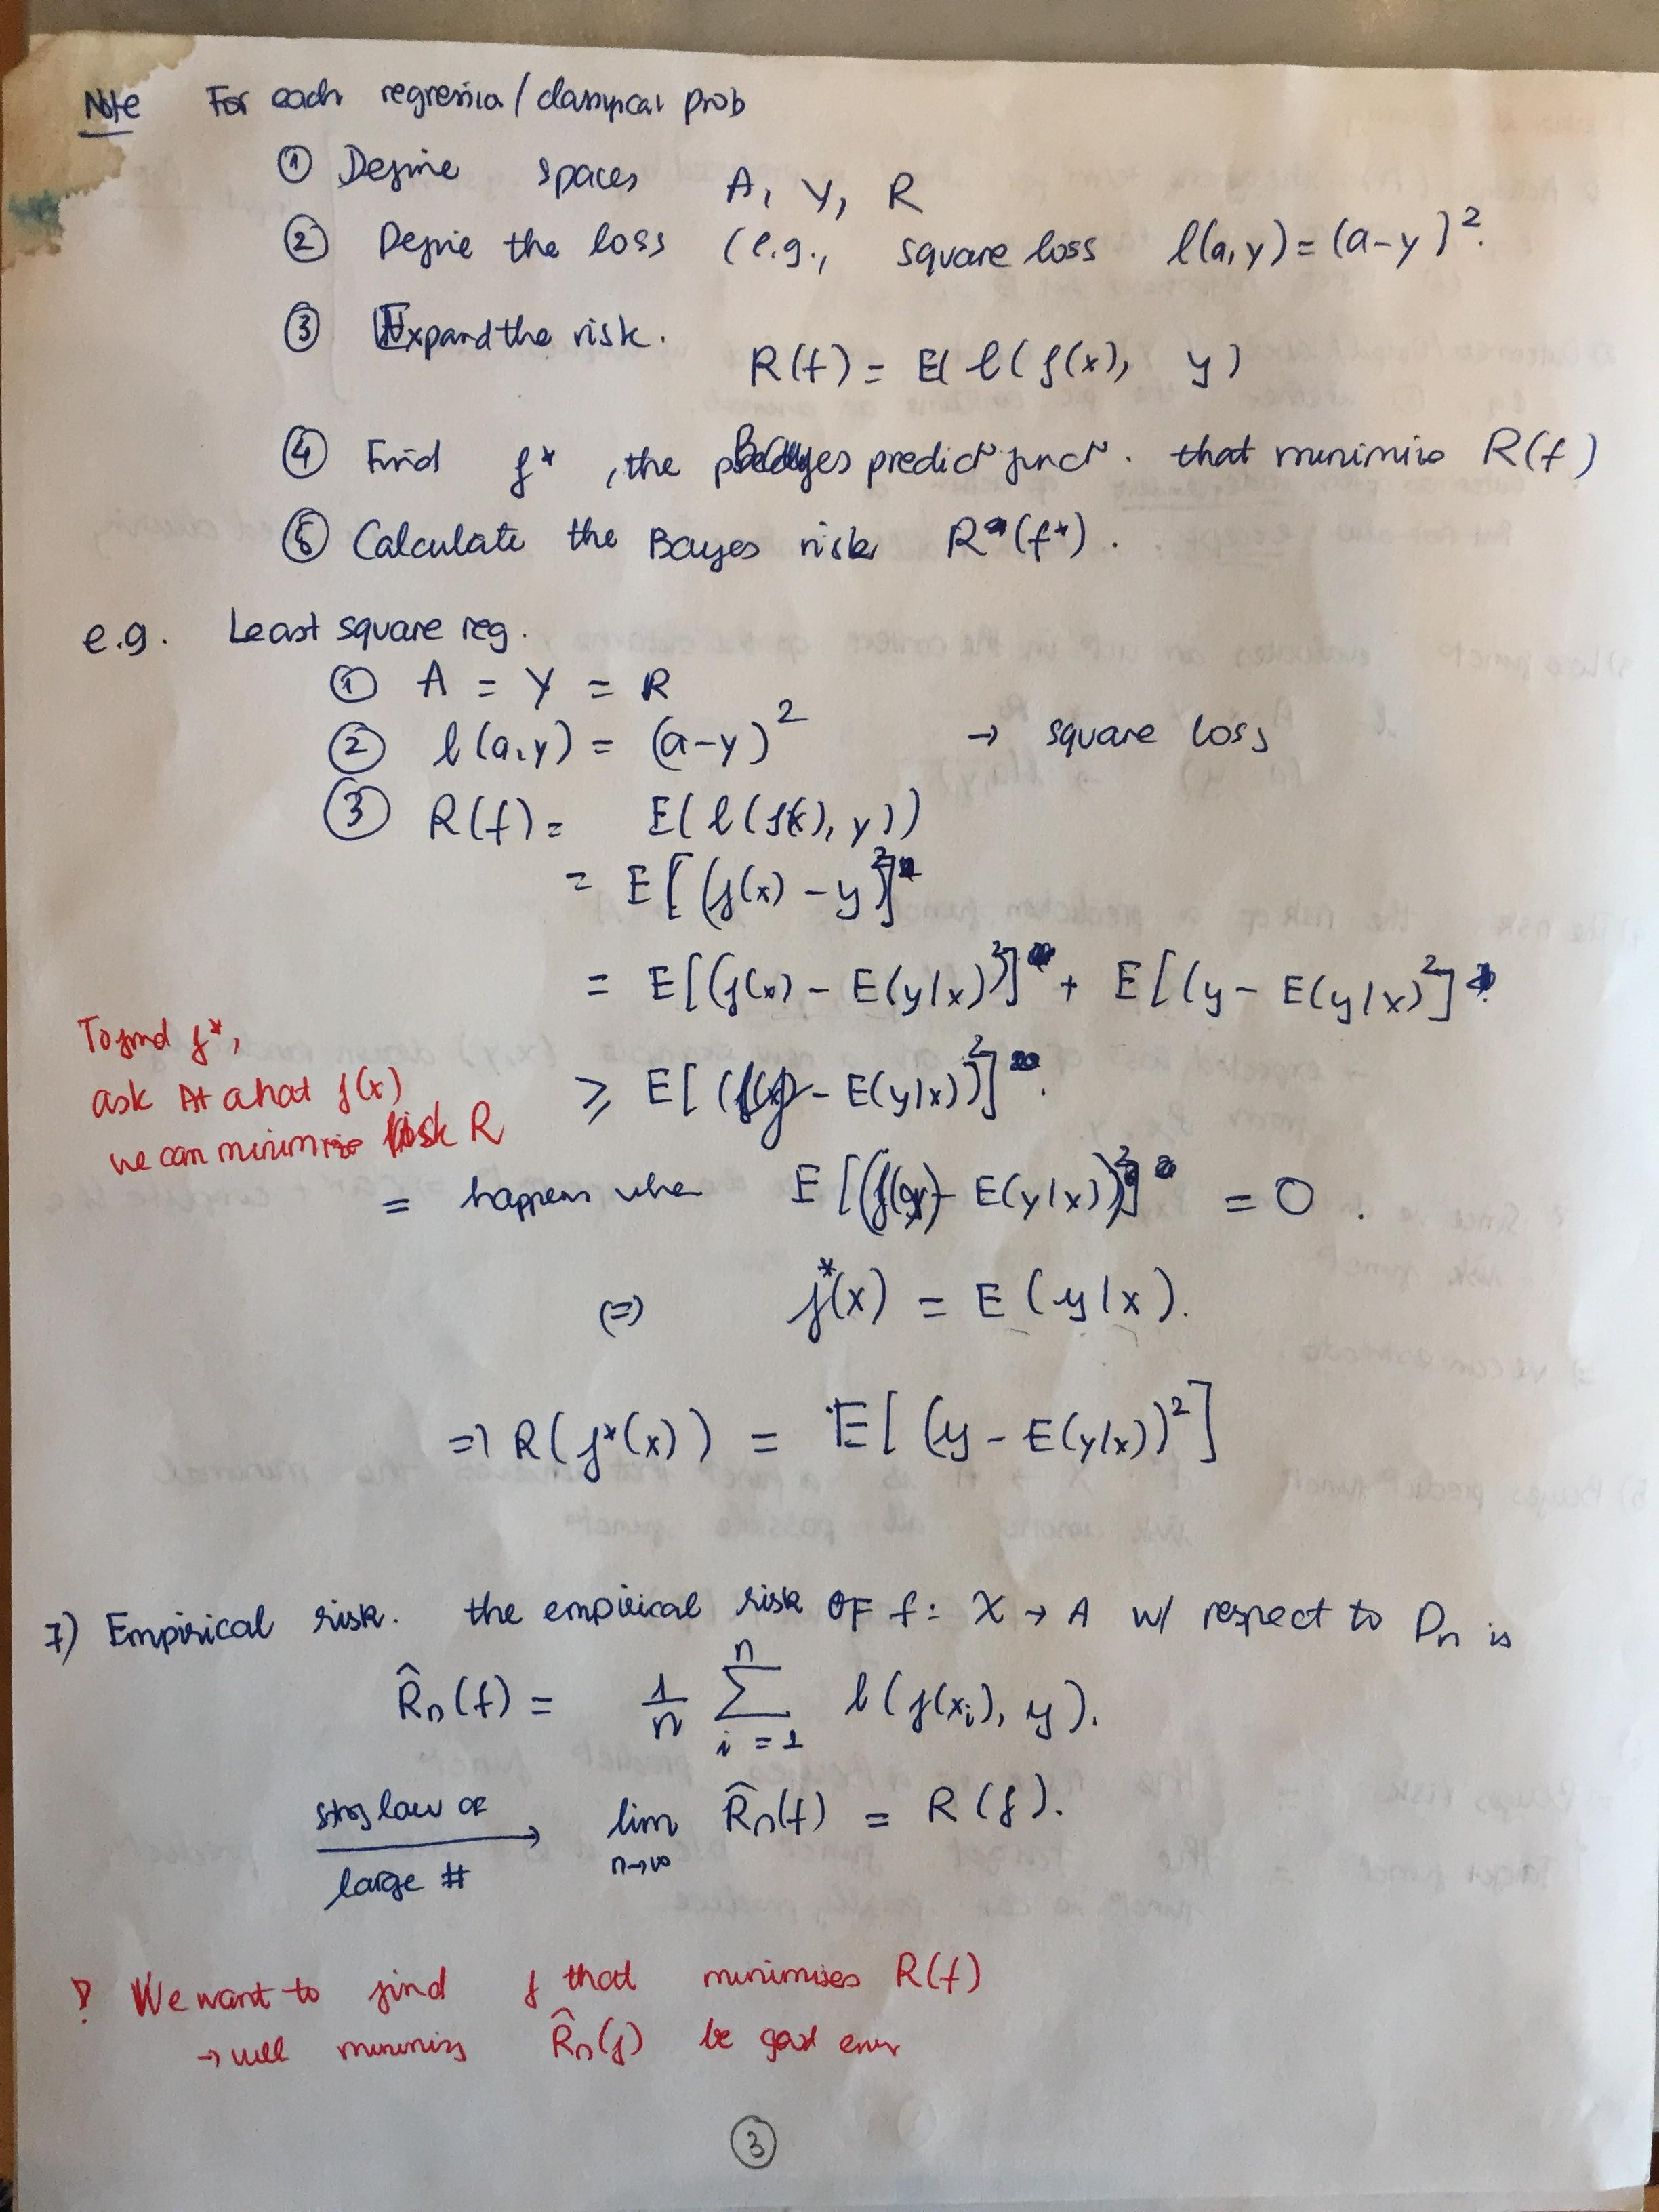
\includegraphics[max size={\textwidth}{\textheight}]{HypoSpace3.jpg} \\
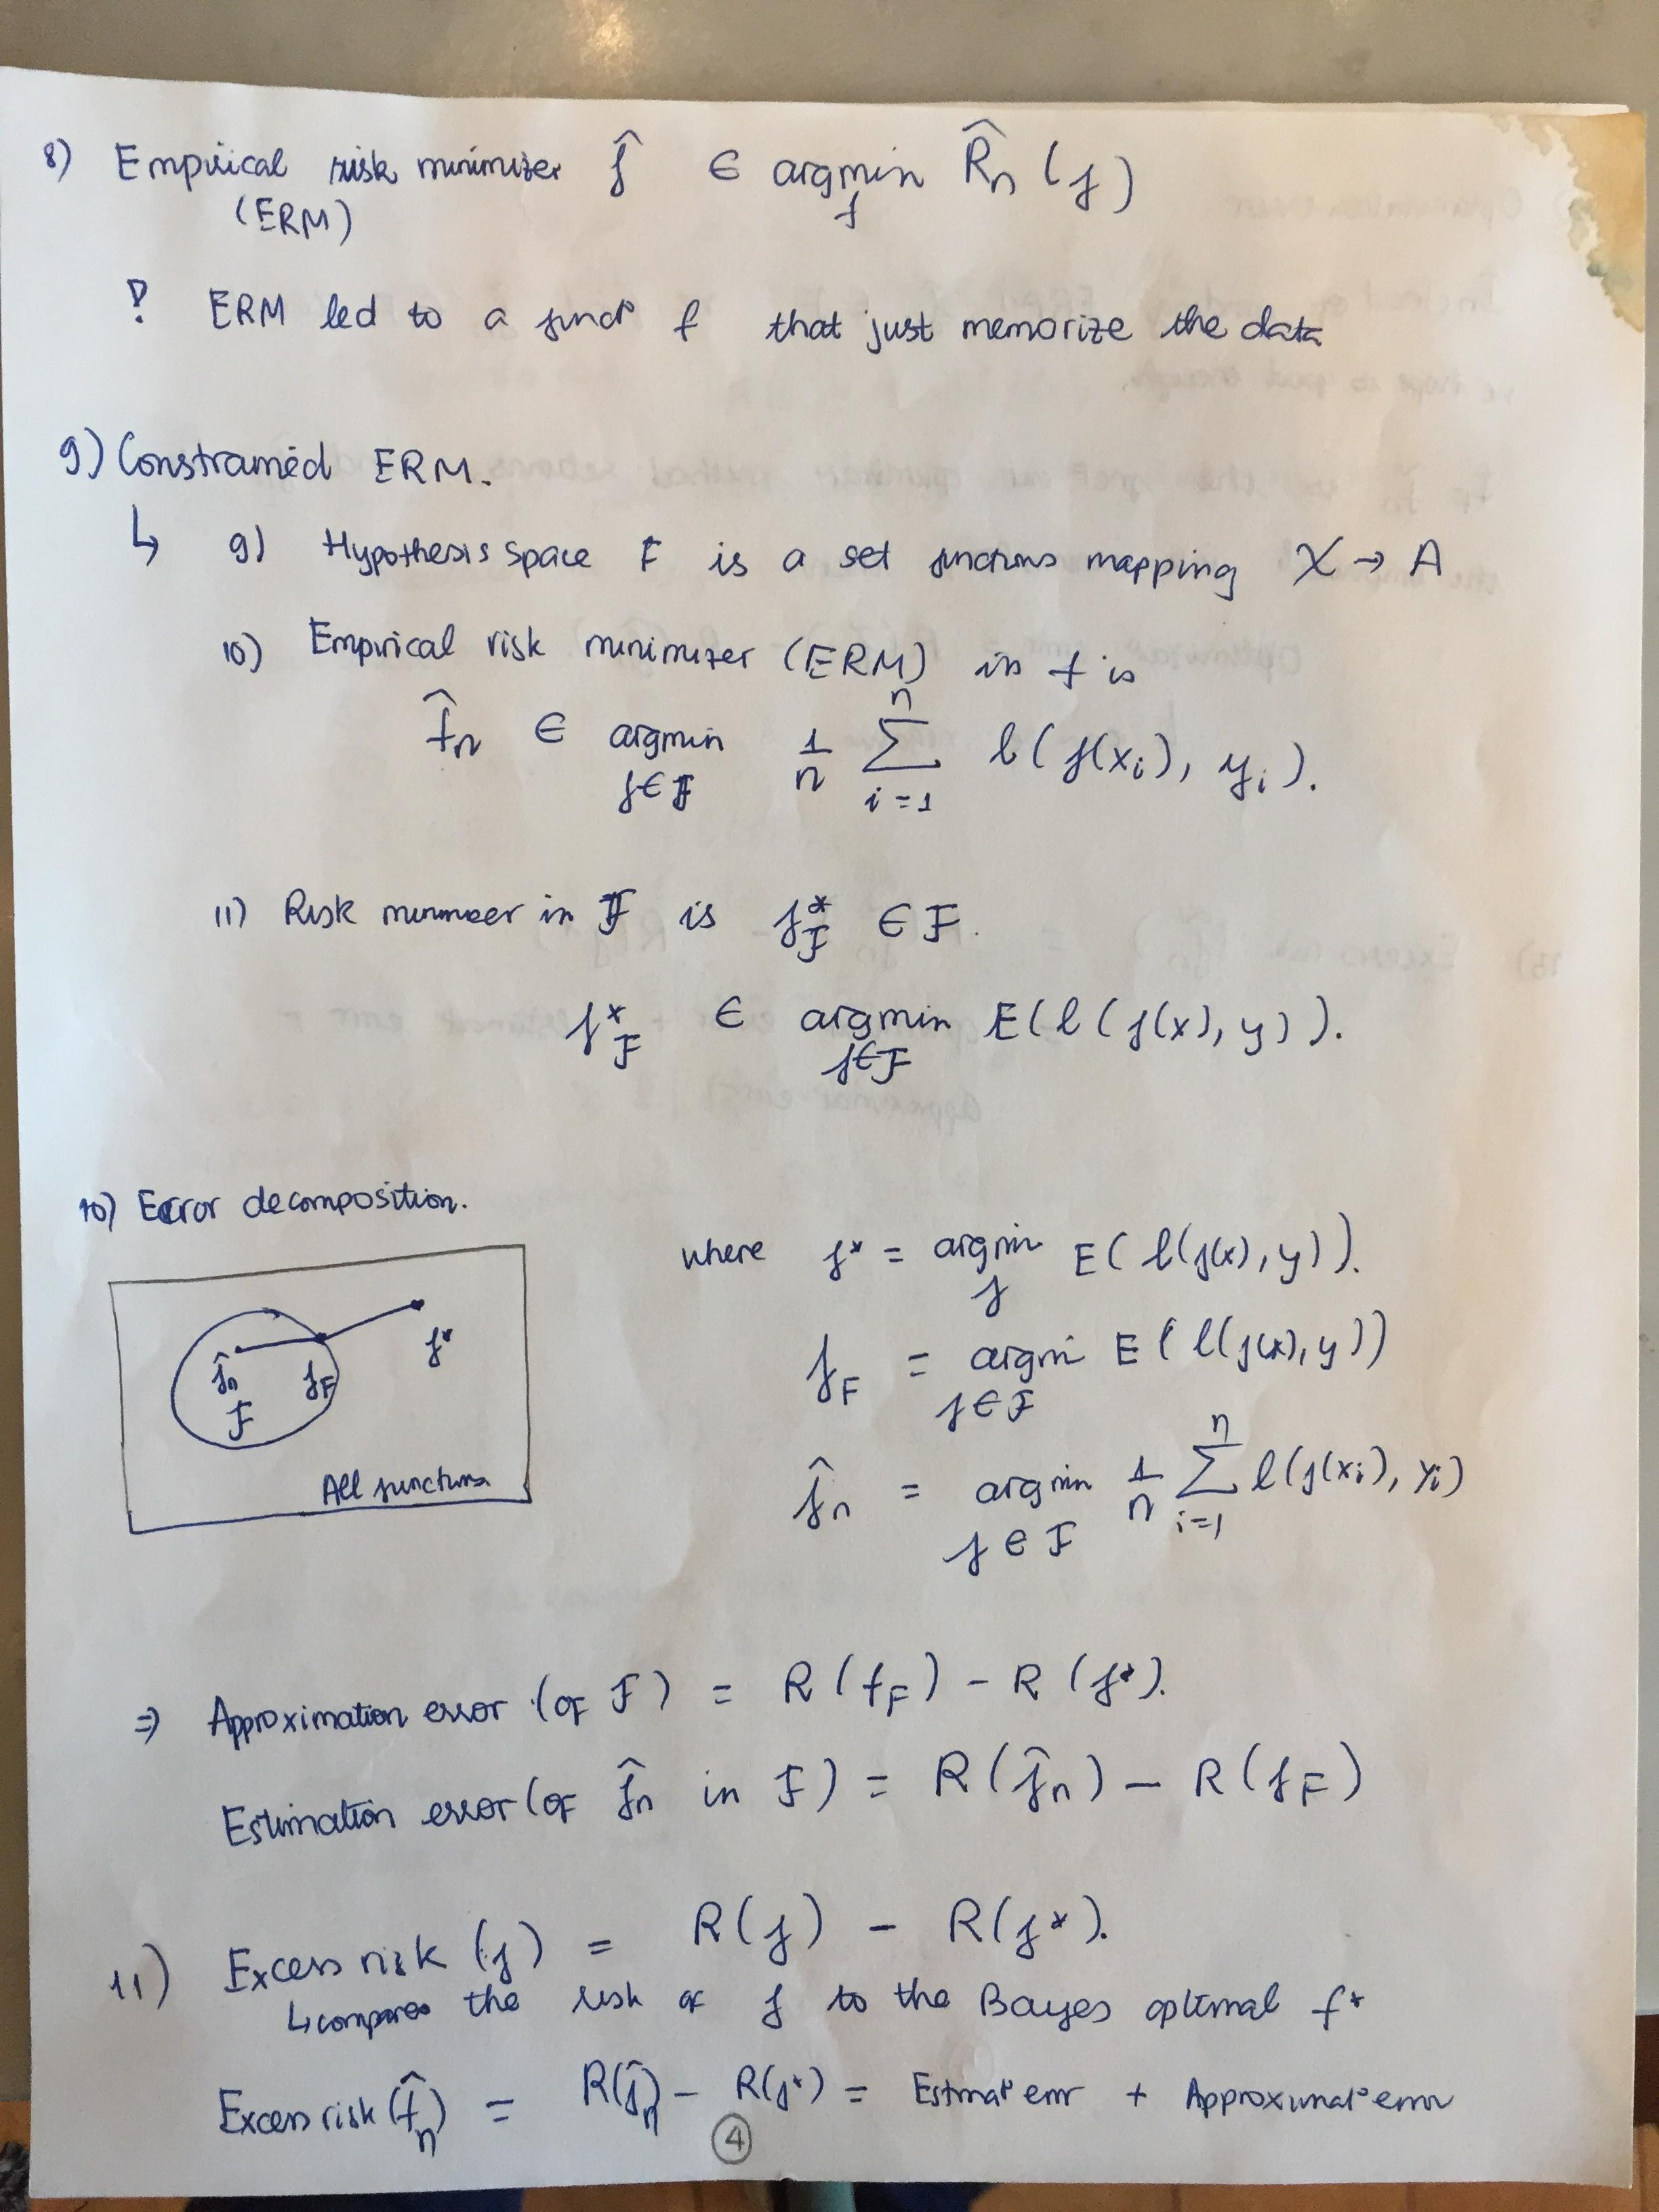
\includegraphics[max size={\textwidth}{\textheight}]{HypoSpace4.jpg} \\

\includepdf[pages=2-,pagecommand={},width=\textwidth]{1-Lec-Check_sol.pdf}
 
\section{Mathematical Fundamentals}
The following questions are designed to check how prepared you are to take this class. Familiarity with linear algebra and probability at the level of these questions is expected for the class.  

\subsection{Probability}
Let $(X_1, X_2, \cdots, X_d)$ have a $d$-dimensional multivariate Gaussian distribution, with mean vector $\mu \in \reals^d$ and covariance matrix $\Sigma \in \reals^{d \times d}$, i.e. $(X_1, X_2, \cdots, X_d)\sim \cn (\mu, \Sigma)$ Use $\mu_i$ to denote the $i^{th}$ element of $\mu$ and $\Sigma_{ij}$ to denote the element at the $i^{th}$ row and $j^{th}$ column of $\Sigma$. 
\begin{enumerate}
\item Let $x, y \in \reals^d$ be two independent samples drawn from $\cn (\mu, \Sigma)$. Give expression for $\ex \|x\|_2^2$ and $\ex \|x-y\|_2^2$. Express your answer as a function of $\mu$ and $\Sigma$. $\|x\|_2$ represents the $L2$-norm of vector $x$.


\item Find the distribution of $Z = \alpha_i X_i + \alpha_j X_j$, for $i\neq j$ and $1 \leq i, j \leq d$. The answer will belong to a familiar class of distribution. Report the answer by identifying this class of distribution and specifying the parameters.

\item (Optional) Assume $W$ and $R$ are two Gaussian distributed random variables. Is $W+R$ still Gaussian? Justify your answer.
\end{enumerate}

\subsection{Linear Algebra}
\begin{enumerate}
\item Let $A$ be a $d\times d$ matrix with rank $k$.  Consider the set $S_A:=\{x \in \reals^d|Ax = 0\}$. What is the dimension of $S_A$?
\item Assume $S_v$ is a $k$ dimensional subspace in $\reals^d$ and $v_1,v_2,\cdots, v_k$ form an orthonormal basis of $S_v$. Let $w$ be an arbitrary vector in $\reals^d$. Find 
\[
x^* = \underset{x\in S_v}{\text{argmin}}\|w-x\|_2,
\]
where $\|w-x\|_2$ is the Euclidean distance between $w$ and $x$. Express $x^*$ as a function of $v_1, v_2, \dots, v_k$ and $w$.

\item (Optional) Continuing from above, $x^*$ can be expressed as 
\[
x^* = Mw,
\]
where $M$ is a $d\times d$ matrix. Prove that such an $M$ always exists or  more precisely find an expression for $M$ as a function of $v_1,v_2,\cdots, v_k$. Compute the eigenvalues and one set of eigenvectors of $M$ corresponding to the nonzero eigenvalues.
\end{enumerate}


\section{Risk Minimization}

\subsection{Square Loss}

\global\long\def\E{\ex}
\begin{enumerate}
\item Let $y$ be a random variable with a known distribution, and consider
the square loss function $\ell(a,y)=(a-y)^{2}$. We want to find the
action $a^{*}$ that has minimal risk. That is, we want to find $a^{*}=\argmin_{a}\ex\left(a-y\right)^{2}$,
where the expectation is with respect to $y$. Show that $a^{*}=\ex y$,
and the Bayes risk (i.e. the risk of $a^{*}$) is $\var(y)$. In other
words, if you want to try to predict the value of a random variable,
the best you can do (for minimizing expected square loss) is to predict
the mean of the distribution. Your expected loss for predicting the
mean will be the variance of the distribution. {[}Hint: Recall that
$\var(y)=\ex y^{2}-\left(\ex y\right)^{2}$.{]}
\item Now let's introduce an input. Recall that the \textbf{expected loss
}or \textbf{``risk''}\emph{ }of a decision function $f:\cx\to\ca$
is
\[
R(f)=\ex\loss(f(x),y),
\]
where $(x,y)\sim P_{\cx\times\cy}$, and the \textbf{Bayes decision
function} $f^{*}:\cx\to\ca$ is a function that achieves the \emph{minimal
risk} among all possible functions: 
\[
R(f^{*})=\inf_{f}R(f).
\]
Here we consider the regression setting, in which $\ca=\cy=\reals$.
We will show for the square loss $\ell(a,y)=\left(a-y\right)^{2}$,
the Bayes decision function is $f^{*}(x)=\ex\left[y\mid x\right]$,
where the expectation is over $y$. As before, we assume we know the
data-generating distribution $P_{\cx\times\cy}$.
\begin{enumerate}
\item We'll approach this problem by finding the optimal action for any
given $x$. If somebody tells us $x$, we know that the corresponding
$y$ is coming from the conditional distribution $y\mid x$. For a
particular $x$, what value should we predict (i.e. what action $a$
should we produce) that has minimal expected loss? Express your answer
as a decision function $f(x)$, which gives the best action for any
given $x$. In mathematical notation, we're looking for $f^{*}(x)=\argmin_{a}\ex\left[\left(a-y\right)^{2}\mid x\right]$,
where the expectation is with respect to $y$. (Hint: There is really
nothing to do here except write down the answer, based on the previous
question. But make sure you understand what's happening...)
\item In the previous problem we produced a decision function $f^{*}(x)$
that minimized the risk for each $x$. In other words, for any other
decision function $f(x)$, $f^{*}(x)$ is going to be at least as
good as $f(x)$, for every single $x$. In math, we mean
\[
\ex\left[\left(f^{*}(x)-y\right)^{2}\mid x\right]\le\ex\left[\left(f(x)-y\right)^{2}\mid x\right],
\]
for all $x$. To show that $f^{*}(x)$ is the Bayes decision function,
we need to show that 
\[
\ex\left[\left(f^{*}(x)-y\right)^{2}\right]\le\ex\left[\left(f(x)-y\right)^{2}\right]
\]
for any $f$. Explain why this is true. (Hint: Law of iterated expectations.)
\end{enumerate}
\end{enumerate}

\subsection{Median Loss}
\begin{enumerate}
\item  Show that for the absolute loss $\ell(\hat{y},y)=\left|y-\hat{y}\right|$,
$f^{*}(x)$ is a Bayes decision function if $f^{*}(x)$ is the median
of the conditional distribution of $y$ given $x$. {[}Hint: As in
the previous section, consider one $x$ at time. It may help to use
the following characterization of a median: $m$ is a median of the
distribution for random variable $y$ if $\pr(y\ge m)\ge\frac{1}{2}$
and $\pr(y\le m)\ge\frac{1}{2}$.{]} Note: This loss function leads
to ``median regression''. There are other loss functions that lead
to ``quantile regression'' for any chosen quantile. (For partial
credit, you may assume that the distribution of $y\mid x$ is discrete
or continuous. For full credit, no assumptions about the distribution.)
\end{enumerate}

\end{document}
